\chapter{Założenia projektowe}
\section{Wykorzystane narzędzia}
W tej części pracy będą opisane narzędzia, które zostały wykorzystane podczas tworzenia projektu. Część z nich była wykorzystana bezpośrednio do tworzenia kodu projektu (np. wybrany język programowania, system budowania czy framework do testowania), niektóre pełniły pomocniczą rolę (np. narzędzie do generowania dokumentacji).

\subsection{Język programowania}
Projekt BBS został zrealizowany w języku C++ standardu C++17.

C++ to uniwersalny język programowania, który łączy wydajność niskopoziomowego C z zaletami programowania obiektowego. Umożliwia tworzenie zarówno prostych, jak i bardzo złożonych systemów, co czyni go popularnym wyborem w takich dziedzinach jak gry, systemy operacyjne, oprogramowanie osadzone i aplikacje wymagające wysokiej wydajności. Dzięki wsparciu dla obiektowości, C++ pozwala na lepszą organizację kodu i zarządzanie złożonymi strukturami. Jednocześnie, umożliwia precyzyjną kontrolę nad pamięcią i zasobami, co jest kluczowe w aplikacjach, gdzie wydajność ma największe znaczenie. Standardowa biblioteka STL dodatkowo ułatwia pracę, oferując gotowe struktury danych i algorytmy.

C++17 (czyli standard, wykorzystany podczas napisania BBS) to wersja języka C++, która wprowadza liczne usprawnienia zwiększające wygodę kodowania i wydajność programów. W standardzie C++17 pojawiły się nowe narzędzia, które ułatwiają programowanie, jak np. \texttt{std::optional}, pomagający w obsłudze wartości opcjonalnych, oraz \texttt{std::variant}, umożliwiający przechowywanie wielu typów w jednej zmiennej. Standard ten wprowadza też udoskonalenia w zakresie optymalizacji kodu, dzięki czemu aplikacje mogą działać szybciej i sprawniej. Zawiera także nowe algorytmy w STL, które skracają czas potrzebny na pisanie i testowanie kodu. 

\subsubsection{Biblioteka języka}
W ramach pracy intensywnie korzystałem z biblioteki standardowej języka C++. Oto są najczęściej używane biblioteki, na bazie których powstał projekt BBS:

\begin{itemize}
    \item \texttt{string} - operacje na ciągach tekstowych; najczęściej wykorzystane podczas przetwarzania danych z plików wejściowych do postaci tokenów, 
    \item \texttt{vector} - do dynamicznego przechowywania danych; kontener jest częścią kodu służącego do przetwarzania danych wejściowych do postaci tokenów, a także wykorzystany do przechowywania danych o plikach i katalogach projektu, 
    \item \texttt{map} - do dynamicznego przechowywania danych; jest bazą funkcji, które odpowiadają za mechanizm zmiennych,
    \item \texttt{optional} - do przechowywania wartości opcjonalnych; służy najczęściej do przetwarzania danych wejściowych, 
    \item \texttt{algorithms} - do sprawnego przetwarzania danych; biblioteka wykorzystana jest jedynie do przetwarzania tokenów do postaci tekstowej w celu wyświetlenia ich wartości gdy program napotka na błędy,
    \item \texttt{filesystem} - do obsługi operacji na plikach i ścieżkach systemowych; na tej bibliotece opera się mechanizm przyspieszenia budowania projektu przez ignorowanie już istniejących plików, 
    \item \texttt{fstream} - do odczytu i zapisu plików,
    \item \texttt{memory} - inteligentne wskaźniki, za pomocą których udało się ograniczyć ryzyko wycieków pamięci i lepiej określić relacje pomiędzy klasami.
\end{itemize}

\subsubsection{Biblioteki zewnętrzne}
Projekt, który powstał podczas pisania tej pracy dyplomowej, nie korzysta z żadnych zewnętrznych bibliotek, oprócz framework'u do testowania (który jest opisany poniżej), głównie dlatego, że został wykorzystany standard C++17. 

W przypadku, gdyby wymagania projektowe ograniczały możliwości wykorzystania nowszych standardów języka C++, do napisania tego samego kodu niezbędnym by było podłączenie biblioteki Boost (zawiera w sobie m.in. funkcje, które obecnie są w nagłówku \texttt{filesystem} albo \texttt{optional}).

\subsection{System budowania}
Do zarządzania procesem budowania projektu wybrałem CMake, który umożliwia łatwą konfigurację kompilacji oraz automatyczne zarządzanie zależnościami. Skoro jest on wielosystemowym, CMake pozwala na płynne dostosowanie budowania do różnych platform oraz integrację z zewnętrznymi bibliotekami przez korzystanie z dobrze opisanych funkcji i zmiennych.

W moim projekcie istnieje jeden główny plik \texttt{CMakeLists.txt}, który zawiera definicję plików źródłowych oraz katalogu plików nagłówkowych, oraz niezbędne klucze kompilatora. Osobno także dodałem możliwość kompilacji testów, która zależy od trybu budowania projektu (\texttt{DEBUG} czy \texttt{RELEASE}).

Testy mają inną strukturę : są one podzielone na osobne, izolowane podprojekty, każdy z których zawiera swój \texttt{CMakeLists.txt}, na które wskazują inne pliki wyższego rzędu.

\subsection{Kompilator}
Do kompilacji projektu użyłem kompilatora GCC 14, który w pełni wspiera standard C++17 i dostarcza narzędzi optymalizujących generowany kod.

GCC \eng{\textbf{G}NU \textbf{C}ompiler \textbf{C}ollection} -- to open-source kompilator wspierający wiele języków programowania. Jest jednym z najpopularniejszych kompilatorów na świecie, głównie ze względu na swoją niezawodność, wydajność i szeroką kompatybilność z różnymi systemami operacyjnymi, takimi jak Linux, Windows, i macOS. 

GCC cechuje się modularną budową, co oznacza, że każdy jego komponent odpowiada za kompilację innego języka programowania lub realizację konkretnego etapu procesu kompilacji. Dzięki tej modularności, GCC obsługuje wiele języków, takich jak C, C++, Fortran czy Ada, z osobnymi frontendami (czyli modułami wstępnie przetwarzającymi kod), które przekształcają kod źródłowy na wspólną reprezentację pośrednią. Następnie, backend kompilatora dokonuje optymalizacji tej reprezentacji i generuje kod maszynowy dostosowany do architektury docelowego procesora.

\subsection{Testowanie}
W celu zapewnienia jakości i poprawności kodu wykorzystałem framework Google Test do tworzenia testów jednostkowych. Testy pozwalają na automatyczne sprawdzanie poprawności funkcji oraz łatwiejsze wykrywanie i naprawę błędów.

Google Test (GTest) to framework do testowania jednostkowego napisany w języku C++. Jego struktura opiera się na kilku głównych komponentach:

\begin{enumerate}
    \item Moduł testowy - Najważniejszy element, który zarządza definiowaniem i organizacją testów. W każdym pliku testowym tworzysz przypadki testowe i grupy testów, co pozwala na logiczne segregowanie testów w obrębie kodu.
    \item Assertions - GTest oferuje szeroką gamę asercji (np. \texttt{ASSERT\_EQ}, \texttt{EXPECT\_TRUE}), które sprawdzają zgodność wyników testów z oczekiwanymi wartościami. Asercje są centralnym modułem GTest i są realizowane jako makra, co ułatwia wywoływanie ich bez skomplikowanej składni. Moduł ten obsługuje różne poziomy asercji, od ostrzeżeń po przerywanie testu w przypadku błędu.
    \item Runner testów - Uruchamianie testów odbywa się przez specjalny runner, który iteruje przez wszystkie przypadki testowe i rejestruje wyniki, pozwala na ponowne odpalenie nieudanych testów. Runner ten jest niezależny od definicji testów, co umożliwia równoczesne lub selektywne uruchamianie wybranych zestawów testów. 
    \item Wyniki - Moduł odpowiedzialny za raportowanie wyników oferuje różne formaty, w tym XML, co ułatwia integrację z innymi narzędziami do analizy wyników testów. Pozwala na szczegółowe monitorowanie i analizę wyników w środowiskach CI/CD.
\end{enumerate}

Ten framework został wybrany do testowania BBS, ponieważ to jest jeden z najbardziej rozpowszechnionych framework'ów, który korzysta z C++, a także jest bardzo prosty, wygodny i potężny.

\subsection{Dokumentacja}
Dokumentacja projektu została wygenerowana przy użyciu narzędzia Doxygen, co pozwoliło na uzyskanie przejrzystej dokumentacji API wraz z automatycznie generowanymi diagramami klas, co ułatwia analizę struktury projektu.

Doxygen to narzędzie do automatycznego generowania dokumentacji z komentarzy w kodzie źródłowym, które wspiera różne języki programowania, w tym C++. Umożliwia ono tworzenie szczegółowych raportów, które opisują strukturę kodu, funkcje, klasy oraz ich wzajemne zależności. Dzięki specjalnym komentarzom w kodzie, Doxygen zbiera informacje o elementach programu, które następnie przekształca w zorganizowaną dokumentację.

Narzędzie generuje dokumentację w różnych formatach, takich jak HTML, LaTeX, PDF czy XML, a także oferuje możliwość tworzenia diagramów klas i zależności między modułami. Używając Doxygen, można w łatwy sposób wygenerować interaktywną dokumentację, która zawiera opisy funkcji, metod oraz struktur danych, a także umożliwia przeglądanie zależności pomiędzy poszczególnymi elementami kodu.

Konfiguracja jednak nie jest aż tak prosta, ponieważ aby wymusić poprawne zachowanie narzędzia jest potrzebna zmiana pliku konfiguracyjnego, zawierająca tysiące linii. Z kolei każdy parametr jest dobrze opisany, więc potrzeba tylko poświęcić jakiś czas zapoznaniu się z narzędziem.

\subsection{Tekst pracy}
Cała część tekstowa pracy dyplomowej została napisana w LaTeX-u. Użycie tego systemu składania tekstu pozwoliło na uzyskanie profesjonalnego i spójnego formatu dokumentu, szczególnie przydatnego przy generowaniu równań, tabel oraz bibliografii.

LaTeX to system, który umożliwia tworzenie zgodnych z pewnym szablonem dokumentów. W LaTeX-u, zamiast zwykłego tekstu, opisuje się strukturę dokumentu i jego formatowanie za pomocą specjalnych poleceń.

Jedną z najważniejszych cech LaTeX jest tworzenie równań, tabel, wykresów i zarządzanie bibliografią. Także LaTeX automatycznie zajmuje się numerowaniem stron, tworzeniem spisów treści i cytowaniami (jeśli są podłączone specjalne biblioteki, których jest mnóstwo), co czyni go idealnym narzędziem do pisania dokumentów technicznych i naukowych, takich jak prace dyplomowe.

\section{Wymagania projektowe}
 Wymagania do projektu/systemu mogą być funkcjonalne lub niefunkcjonalne.

Przed rozpoczęciem pracy nad projektem bardzo ważne jest określić wymagania, ponieważ bez tego śledzenie procesu wykonania zadań jest niemożliwe. Określenie wymagań to kluczowy etap w cyklu życia każdego systemu lub oprogramowania. Podczas trwania tego etapu tworzony jest szczegółowy zestaw wymagań zgodny z celami, jakie ma realizować przyszły system. Proces ten jest złożony, często podatny na błędy.

Ten etap  ma szczególne znaczenie, ponieważ dobrze określone wymagania stanowią fundament całego projektu i decydują o jego sukcesie. Błędy popełnione na tym etapie są niezwykle kosztowne, skoro naprawa "fundamentu" projektu jest trudna, czasochłonna i bardzo niebezpieczna z punktu widzenia jakości oraz planowania.

\subsection{Wymagania funkcjonalne}
Wymagania funkcjonalne to specyfikacje, które precyzują, co dokładnie system ma realizować, skupiając się na zadaniach i funkcjach, które użytkownik będzie mógł wykonywać. Opisują one konkretne operacje i reakcje systemu na działania użytkownika, definiując jego oczekiwane zachowanie w różnych sytuacjach.

Poniżej znajdują się wymagania funkcjonalne dla projektu ,,Better Build System''.
\begin{enumerate}
    \item System powinien obsługiwać kompilację kodu C++, zarówno dla pojedynczych plików źródłowych, jak i całych modułów, 
    \item System powinien zapewniać obsługę wieloetapowej kompilacji dla dużych projektów (czyli plik źródłowy $\rightarrow$ plik obiektowy $\rightarrow$ plik wykonywalny).
    \item System powinien umożliwiać automatyczne linkowanie plików obiektowych, tworząc gotowe pliki wykonywalne na podstawie podanej informacji.
    \item System powinien monitorować zależności między plikami źródłowymi, by kompilować tylko te, które zostały zmodyfikowane albo mają zmodyfikowane zależności
    \item System powinien dostawać informację o projektach do budowania z plików konfiguracyjnych.
    \item System powinien generować przejrzyste komunikaty z informacjami miejscach wystąpienia błędów wraz z ich opisem.
    \item System powinien mieć możliwość wykonywania wprowadzonych przez użytkownika komend przed oraz po kompilacji.
    \item System powinien zapewniać możliwość zmiany nazwy projektu oraz nazwy pliku wykonywalnego.
    \item System powinien zapewniać możliwość zmiany parametrów kompilacji i linkowania.
\end{enumerate}

\subsection{Wymagania niefunkcjonalne}
Wymagania niefunkcjonalne odnoszą się do tego, jak system ma działać i jakie standardy powinien spełniać. Skupiają się na jakościowych aspektach systemu, które decydują o jego efektywności i satysfakcji użytkowników, ale nie są bezpośrednio związane z funkcjami użytkowymi. Faktycznie, to są ograniczenia, przy zachowaniu których system będzie działał w prawidłowy sposób.

Poniżej są wymienione wymagania niefunkcjonalne dla projektu "Better Build System".
\begin{enumerate}
    \item \textbf{Wydajność}: System powinien efektywnie zarządzać zależnościami, aby uniknąć niepotrzebnej rekompilacji.
    \item \textbf{Niezawodność}: BBS musi działać stabilnie i obsługiwać duże ilości kodu bez awarii. W przypadku błędów kompilacji lub testów, powinien przekazywać czytelne komunikaty.
    \item \textbf{Łatwość użytkowania}: Konfiguracja programu powinny być intuicyjne. Dokumentacja oraz komunikaty powinny być jasne, a konfiguracja wymagać minimalnej ilości kroków.
    \item \textbf{Przenośność i kompatybilność}: System powinien działać na różnych platformach (Linux, Windows, macOS), wspierając popularne kompilatory (szczególnie GCC). Wykorzystywane technologie i narzędzia powinny być kompatybilne z językiem C++17, a sam projekt musi być zarządzany za pomocą wieloplatformowego systemu budowania (w tym przypadku CMake).
    \item \textbf{Modularność i elastyczność}: Architektura systemu musi być modularna, aby umożliwić łatwe dodawanie nowych funkcji i wsparcie dla kolejnych narzędzi czy technologii. Każda klasa musi być w osobnym pliku oraz w module, który nazywa się tak samo jak i katalog, w którym znajduje się plik.
    \item \textbf{Integracja z innymi narzędziami}: BBS powinien łatwo integrować się z systemami zarządzania wersjami (jak Git) oraz narzędziami do testowania (Google Test) i dokumentacji (Doxygen), wspierając typowy proces rozwoju oprogramowania.
    \item \textbf{Skalowalność}: System musi być skalowalny, aby efektywnie obsługiwać zarówno małe, jak i rozbudowane projekty C++ bez utraty wydajności i stabilności. Podstawą do tego służy napisanie kodu zgodnie z zasadami OOP i SOLID
    \item \textbf{Bezpieczeństwo}: BBS powinien chronić integralność plików źródłowych, nie modyfikując ich bez wyraźnej instrukcji użytkownika.
    \item \textbf{Wysoka jakość kodu}: Kod źródłowy systemu powinien być napisany zgodnie z zasadami OOP oraz SOLID, poprawnie formatowany za pomocą narzędzia clang-format i być zgodny z Google Styleguide.
    \item \textbf{Dostępność dokumentacji}: System musi umożliwiać łatwe generowanie dokumentacji projektu przy użyciu narzędzia Doxygen. Dokumentacja powinna być pełna i wyczerpująca, opisując zarówno instalację, konfigurację, jak i wszystkie funkcje BBS, by użytkownicy mogli szybko uzyskać potrzebne informacje. Dokumentacja musi być dostępna w kilku formatach: HTML, XML, PDF.
\end{enumerate}

\subsection{Przypadki użycia}
\begin{figure}[h]
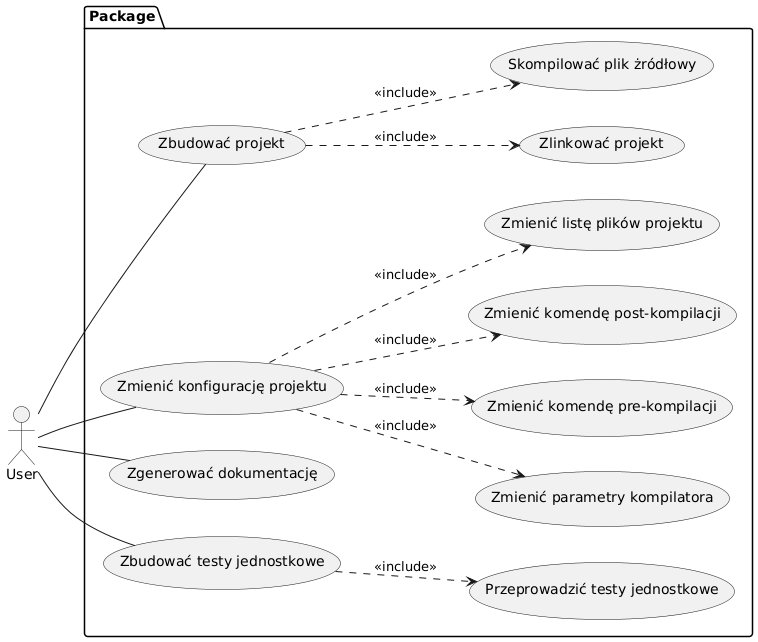
\includegraphics[width=\textwidth]{Images/use-case.png}
\end{figure}

Oprócz wymagań muszą być opisane przypadki użycia programu. Przypadki użycia opisują sekwencje interakcji pomiędzy aktorem (użytkownikiem), a systemem. One są ściśle powiązane z wymaganiami projektowymi i pozwalają wdrożyć tylko i wyłącznie potrzebne funkcje, odrzucając wszystkie inne niewykorzystane funkcje.

Takie podejście nie tylko pozwala usunąć zbędne funkcje, skracając czas realizacji projektu i zmniejszając koszt jego tworzenia, ale też skupia się na użytkownikach.

\subsection{Zbudować projekt (UC1)}
\begin{itemize}
    \item Cel: Umożliwić użytkownikowi pełne zbudowanie projektu, które obejmuje kompilację wszystkich plików źródłowych oraz ich późniejsze połączenie w jeden wynikowy plik wykonywalny lub bibliotekę.
    \item Warunki początkowe: Projekt zawiera poprawnie skonfigurowane pliki źródłowe oraz ustawienia kompilacji.
    \item Warunki końcowe: Projekt został zbudowany.
\end{itemize}

\subsubsection{Scenariusz}
\begin{itemize}
    \item Użytkownik uruchamia program z podaniem pliku konfiguracyjnego.
    \item System rozpoczyna kompilację plików źródłowych, uruchamiając przypadek użycia „Skompilować plik źródłowy”.
    \item System przeprowadza proces linkowania, uruchamiając przypadek „Zlinkować projekt”.
    \item W przypadku braku błędów budowania system zwraca wynikowy plik wykonywalny lub bibliotekę.
    \item System informuje użytkownika o pomyślnym zakończeniu budowy lub zgłasza ewentualne błędy.
\end{itemize}

\subsection{Skompilować plik źródłowy (UC2)}
\begin{itemize}
    \item Cel: Umożliwić kompilację pojedynczego pliku źródłowego, przekształcając kod źródłowy na kod maszynowy zrozumiały dla komputera.
    \item Warunki początkowe: Plik źródłowy jest dostępny i poprawnie napisany zgodnie z językiem C++.
    \item Warunki końcowe: Plik został skompilowany.
\end{itemize}

\subsubsection{Scenariusz}
\begin{itemize}
    \item System odczytuje wybrany plik źródłowy.
    \item System stosuje ustalone parametry kompilatora do pliku.
    \item System wykonuje proces kompilacji pliku.
    \item W przypadku sukcesu system generuje skompilowany plik obiektowy, informując użytkownika.
    \item W przypadku błędów kompilacji, system zgłasza błędy.
\end{itemize}

\subsection{Zlinkować projekt (UC3)}
\begin{itemize}
    \item Cel: Połączyć wszystkie skompilowane pliki obiektowe w jeden finalny plik wykonywalny lub bibliotekę.
    \item Warunki początkowe: Projekt zawiera co najmniej jeden skompilowany plik obiektowy.
    \item Warunki końcowe: Projekt został zlinkowany.
\end{itemize}

\subsubsection{Scenariusz}
\begin{itemize}
    \item System odczytuje listę plików obiektowych do linkowania.
    \item System wykonuje proces linkowania, tworząc wynikowy plik.
    \item Jeśli linkowanie zakończy się sukcesem, system generuje plik wynikowy i informuje użytkownika.
    \item Jeśli wystąpią błędy, system zgłasza je użytkownikowi.
\end{itemize}

\subsection{Zmienić konfigurację projektu (UC4)}
\begin{itemize}
    \item Cel: Umożliwić użytkownikowi edycję ustawień projektu, co pozwala na dostosowanie jego konfiguracji.
    \item Warunki początkowe: Projekt jest otwarty i posiada dostępne pliki konfiguracyjne.
    \item Warunki końcowe: Konfiguracja projektu została zaktualizowana.
\end{itemize}

\subsubsection{Scenariusz}
\begin{itemize}
    \item Użytkownik otwiera plik konfiguracji projektu.
    \item Użytkownik dokonuje zmian w wybranych ustawieniach.
    \item Użytkownik zapisuje zmiany w konfiguracji projektu.
\end{itemize}

\subsection{Zmienić listę plików projektu (UC5)}
\begin{itemize}
    \item Cel: Pozwala użytkownikowi dodawać lub usuwać pliki źródłowe albo nagłówkowe wchodzące w skład projektu.
    \item Warunki początkowe: Projekt jest otwarty i zawiera aktualną listę plików źródłowych.
    \item Warunki końcowe: Lista plików zmieniona.
\end{itemize}

\subsubsection{Scenariusz}
\begin{itemize}
    \item Użytkownik otwiera plik konfiguracji projektu.
    \item Użytkownik dodaje lub usuwa pliki.
    \item Użytkownik zapisuje zmiany w konfiguracji projektu.
\end{itemize}

\subsection{Zmienić parametry kompilatora (UC6)}
\begin{itemize}
    \item Cel: Umożliwić użytkownikowi dostosowanie parametrów kompilatora, takich jak poziom optymalizacji, ostrzeżenia i inne ustawienia.
    \item Warunki początkowe: Kompilator jest zainstalowany i dostępny w systemie.
    \item Warunki końcowe: pParametry kompilatora zostały zmienione.
\end{itemize}

\subsubsection{Scenariusz}
\begin{itemize}
    \item Użytkownik otwiera plik konfiguracji projektu.
    \item Użytkownik wprowadza zmiany w ustawieniach.
    \item Użytkownik zapisuje zmiany w konfiguracji projektu.
\end{itemize}

\subsection{Zmienić komendę pre-kompilacji (UC7)}
\begin{itemize}
    \item Cel: Umożliwić użytkownikowi ustawienie komend wykonywanych przed kompilacją, np. generacji kodu lub czyszczenia plików tymczasowych.
    \item Warunki początkowe: Projekt jest otwarty, a użytkownik posiada uprawnienia do edycji konfiguracji.
    \item Warunki końcowe: Komenda została zmieniona.
\end{itemize}

\subsubsection{Scenariusz}
\begin{itemize}
    \item Użytkownik otwiera plik konfiguracji projektu.
    \item Użytkownik wprowadza nowe komendy.
    \item Użytkownik zapisuje zmiany w konfiguracji projektu.
\end{itemize}

\subsection{Zmienić komendę post-kompilacji (UC8)}
\begin{itemize}
    \item Cel: Pozwala użytkownikowi skonfigurować komendy, które zostaną wykonane po zakończeniu kompilacji, np. kopiowanie plików wynikowych.
    \item Warunki początkowe: Projekt jest otwarty, a użytkownik posiada uprawnienia do edycji konfiguracji.
    \item Warunki końcowe: Komenda została zmieniona.
\end{itemize}

\subsubsection{Scenariusz}
\begin{itemize}
    \item Użytkownik otwiera plik konfiguracji projektu.
    \item Użytkownik wprowadza nowe komendy.
    \item Użytkownik zapisuje zmiany w konfiguracji projektu.
\end{itemize}

\subsection{Wygenerować dokumentację (UC9)}
\begin{itemize}
    \item Cel: Umożliwić generację dokumentacji projektu na podstawie kodu źródłowego i komentarzy.
    \item Warunki początkowe: Projekt posiada odpowiednie komentarze i strukturę kodu umożliwiającą generowanie dokumentacji.
    \item Warunki końcowe: Dokumentacja została wygenerowana.
\end{itemize}

\subsubsection{Scenariusz}
\begin{itemize}
    \item Użytkownik uruchamia narzędzie generacji dokumentacji.
    \item Doxygen analizuje kod źródłowy i tworzy dokumentację.
    \item Doxygen zapisuje wygenerowaną dokumentację i informuje użytkownika.
\end{itemize}

\subsection{Zbudować testy jednostkowe (UC10)}
\begin{itemize}
    \item Cel: Umożliwić użytkownikowi zbudowanie testów jednostkowych projektu.
    \item Warunki początkowe: Projekt zawiera pliki testowe zgodne z frameworkiem testowym.
    \item Warunki końcowe: Testy jednostkowe zostały zbudowane.
\end{itemize}

\subsubsection{Scenariusz}
\begin{itemize}
    \item Użytkownik wybiera opcję budowy testów jednostkowych.
    \item System buduje testy jednostkowe.
    \item W przypadku braku błędów budowania, system informuje użytkownika o zakończeniu procesu.
\end{itemize}

\subsection{Przeprowadzić testy jednostkowe (UC11)}
\begin{itemize}
    \item Cel: Umożliwić uruchomienie i weryfikację testów jednostkowych w celu sprawdzenia poprawności kodu.
    \item Warunki początkowe: Testy jednostkowe zostały wcześniej zbudowane i są gotowe do uruchomienia.
    \item Warunki końcowe: Wyniki testów jednostkowych zostały zgłoszone użytkownikowi.
\end{itemize}

\subsubsection{Scenariusz}
\begin{itemize}
    \item Użytkownik wybiera opcję uruchomienia testów jednostkowych.
    \item System wykonuje testy i zbiera ich wyniki.
    \item System raportuje wyniki testów, informując użytkownika o przeprowadzonych testach oraz ich rezultatach (sukces lub błąd).
\end{itemize} 